\documentclass[11pt, a4paper, pdftex, twoside, dvipsnames]{article}
% font:
\usepackage{amsmath,amssymb,amsthm,amsfonts}
\usepackage{bm}  % From amsmath, a bold font
\newcommand{\argmax}{\mathop{\rm arg~max}\limits}
\newtheorem{them}{Theorem}
\newtheorem{prop}{Proposition}
\newtheorem{defn}{Definition}
\everymath{\displaystyle}
\allowdisplaybreaks
\usepackage{mathtools}
\usepackage[makeroom]{cancel}
%\usepackage{newtxtext,newtxmath}
\usepackage[title]{appendix}
\usepackage{epigraph}
% --------------------------------------------------------------------------- %
% figure:
\usepackage[labelfont=bf,font=small]{caption}
%\captionsetup[figure]{name=Fig.,labelsep=space}
%\captionsetup[table]{name=Table\ ,labelsep=space,font=normal}
%\usepackage{subfig}
% \subcaption with {}:
%\captionsetup{subrefformat=parens}
\usepackage{rotating}
\usepackage{float}
\usepackage{graphicx}  % remove 'demo' option for your real document
% --------------------------------------------------------------------------- %
% table

\usepackage{siunitx}
\usepackage[dvipsnames]{xcolor}

\usepackage{threeparttable}
\usepackage{multirow}
\usepackage{multicol}
\usepackage{blkarray}
\usepackage{booktabs}
\usepackage{arydshln}
\usepackage{tabularx}
\usepackage{longtable, array}
\newcolumntype{P}[1]{>{\raggedright\arraybackslash}p{#1}}
\usepackage{tikz}
\usetikzlibrary{arrows.meta}
%\usepackage[dvipsnames]{xcolor}
% --------------------------------------------------------------------------- %
% necessary usepackage
%\usepackage[x11names]{xcolor}
% Hyperref:
\usepackage[bookmarks=false, bookmarksnumbered=true,
colorlinks=true,setpagesize=false,
pdftitle={},pdfauthor={SimonScheidegger},pdfsubject={},
pdfkeywords={}, bookmarkstype=toc, urlcolor=black, citecolor=blue,
linkcolor=black, filecolor=black]{hyperref}


\hypersetup{
    colorlinks=true,
    linkcolor=red,
    filecolor=magenta,      
    urlcolor=cyan
    }


\usepackage{indentfirst}
% \setlength{\parindent}{0pt}
% \setlength{\parskip}{1ex plus 0.5ex minus 0.2ex} 
\usepackage{enumitem}
\usepackage{cases}
\usepackage{url}
\usepackage{setspace}
% \singlespacing
% \doublespacing
\setstretch{1}
\usepackage{ulem}
\usepackage{lscape}
\usepackage{here}
\usepackage{authblk}
\usepackage{framed}
\usepackage{adjustbox}
\usepackage{pdflscape}
\usepackage{listings}
\usepackage{cleveref}
\crefname{equation}{Eq.}{Eqs.}
\crefname{figure}{Figure}{Figures}
\crefname{table}{Table}{Tables}
\crefname{line}{Algorithm}{Algorithms}
\crefname{asmp}{Assumption}{Assumptions}
\crefname{section}{Section}{Sections}
\crefname{chapter}{Chapter}{Chapters}
\crefname{appsec}{Appendix}{Appendixes}
\let\normalref\ref
\renewcommand{\ref}{\cref}
%\usepackage{subcaption}
% \subcaption with {}:
%\captionsetup{subrefformat=parens}


\usepackage[bottom]{footmisc}

%%%%%%%%% Aryan's Macros %%%%%%%%
\DeclareFontFamily{U}{mathx}{}
\DeclareFontShape{U}{mathx}{m}{n}{<-> mathx10}{}
\DeclareSymbolFont{mathx}{U}{mathx}{m}{n}
\DeclareMathAccent{\widehat}{0}{mathx}{"70}
\DeclareMathAccent{\widecheck}{0}{mathx}{"71}
\newcommand{\too}[2]{\text{#1} \! \to \! \text{#2}}
\newcommand{\bb}[1]{\boldsymbol{\bold{#1}}}
\newcommand{\bbh}[1]{\widehat{\boldsymbol{\bold{#1}}}}
\newcommand{\bbb}[1]{\overline{\boldsymbol{\mathrm{#1}}}}
\newcommand{\bbt}[1]{\tilde{\boldsymbol{\mathrm{#1}}}}
\newcommand{\bbv}[1]{\text{vec}({\boldsymbol{\mathrm{#1}}})}
\newcommand{\ekk}[0]{\mathcal{K}}
\newcommand{\spn}[2]{ \text{span}\{#1 \,:\, #2 \}}
\newcommand{\card}[1]{|#1|}
\newcommand{\nnz}[1]{\text{nnz}(#1)}
\newcommand{\abs}[1]{\text{Abs}(#1) }
\newcommand{\maximize}[1]{\underset{ #1 }{\text{max}} }
\newcommand{\argmin}[1]{\underset{#1}{\text{argmin}} }
%\newcommand{\argmax}[1]{\underset{#1}{\text{arg~max}~} }
\newcommand{\minimize}[1]{\underset{ #1 }{\text{min}} }
\newcommand{\subjectTo}[0]{\text{s.t.}\quad }
\newcommand{\nn}{\newline\newline\noindent}
\newcommand{\sign}[1]{\text{sign}(#1)}
\newcommand{\tr}[1]{\text{tr}(#1)}
%%%%%%%%% Aryan's Macros %%%%%%%%

\newcommand{\fixmeAlex}[1]{\textbf{\emph{\textcolor{red}{/* TBD Alex: #1 */}}}}
\newcommand{\fixmeSimon}[1]{\textbf{\emph{\textcolor{blue}{/* TBD Simon: #1 */}}}}
\newcommand{\fixmeFelix}[1]{\textbf{\emph{\textcolor{red}{/* TBD Felix: #1 */}}}}
\newcommand{\fixmeDoris}[1]{\textbf{\emph{\textcolor{red}{/* TBD Doris: #1 */}}}}
\newcommand{\fixmeAryan}[1]{\textbf{\emph{\textcolor{red}{/* TBD Doris: #1 */}}}}
\newcommand{\Question}[1]{\textbf{\emph{\textcolor{red}{/* Question to all: #1 */}}}}

% --------------------------------------------------------------------------- %
% size of the paper: A4
\usepackage[a4paper,left=2cm,right=2cm,top=2.5cm,bottom=2.5cm]{geometry}
% setting for header
\usepackage{fancyhdr}
\pagestyle{fancy}
% \fancyhead[RO,LE]{\thepage}
% \fancyhead[RE,LO]{{\textsf \leftmark}}
% \fancyfoot{}
% \fancyhead[re,lo]{\sffamily\nouppercase{\leftmark}}
\fancyhead[re,lo]{}
\fancyhead[ro,le]{\thepage}
\fancyfoot{}
% for the first page
\fancypagestyle{firstpagestyle}{
\renewcommand{\headrulewidth}{0pt}
\fancyhf{} % clear all header and footer fields
\fancyfoot[C]{\thepage}
}
% for the first page of CV
\fancypagestyle{CVfirstpagestyle}{
\renewcommand{\headrulewidth}{0pt}
\fancyhf{} % clear all header and footer fields
\fancyfoot[C]{\thepage}
}
% --------------------------------------------------------------------------- %
% BibLaTeX with jecon bibliography style
\usepackage{natbib}
\bibliographystyle{jpe}
%-------------------------------------------
% Macros
\renewcommand{\vec}[1]{{\mathbf{#1}}}
\newcommand{\mat}[1]{\underline{\underline{\vec{#1}}}}

% --------------------------------------------------------------------------- %
% rename:
\renewcommand{\refname}{Bibliographies}
\renewcommand{\abstractname}{Abstract}
\newcommand{\defeq}{\mathrel{\mathop:}=}
\newcommand{\eqdef}{\mathrel{\mathop=}:}
\renewcommand{\topfraction}{1.0}
\renewcommand{\bottomfraction}{1.0}
\renewcommand{\dbltopfraction}{1.0}
\renewcommand{\textfraction}{0.01}
\renewcommand{\floatpagefraction}{1.0}
\renewcommand{\dblfloatpagefraction}{1.0}
\setcounter{topnumber}{5}
\setcounter{bottomnumber}{5}
\setcounter{totalnumber}{10}
% --------------------------------------------------------------------------- %
\title{Ocean, land, and atmosphere (OLA): a simple climate emulator for net-zero emission scenarios\thanks{We thank ..., as well as seminar participants at the University of Lausanne and the University of Zurich for very useful conversations and comments. This work was supported by the Swiss National Science Foundation (SNF), under project ID  \lq\lq Can Economic Policy Mitigate Climate-Change?\rq\rq, and for research support. Simon Scheidegger gratefully acknowledges support from the MIT Sloan School of Management.}}
\author{
    Aryan Eftekhari\thanks{TBA, UNI; Email:
    \href{mailto:bla}{bla.ch}.}, \;
    Pratyuksh Bansal\thanks{Institute of Computing, Universit\`a della Svizzera italiana; Email:
    \href{mailto:pratyuksh.bansal@sam.math.ethz.ch}{pratyuksh.bansal@sam.math.ethz.ch}.}, \;
    Doris Folini\thanks{Institute for Atmospheric and Climate Science, ETHZ; Email:
    \href{mailto:doris.folini@env.ethz.ch}{doris.folini@env.ethz.ch}.}, \;
  Felix K\"ubler\thanks{Department for Banking and Finance, University of Z\"urich; Swiss Finance Institute (SFI); Email: \href{mailto:fkubler@gmail.com}{felix.kuebler@bf.uzh.ch}.}, \\ \;
  Aleksandra Malova\thanks{Department of Economics, University of Lausanne; Email: \href{mailto:malova.alex@unil.ch}{aleksandra.malova@unil.ch}.}, \; 
  Simon Scheidegger\thanks{Department of Economics, University of Lausanne; Enterprise for Society (E4S); Email: \href{mailto:simon.scheidegger@unil.ch}{simon.scheidegger@unil.ch}}, \;
  Olaf Schenk\thanks{Institute of Computing, Universit\`a della Svizzera italiana; Email: \href{mailto:olaf.schenk@usi.ch}{olaf.schenk@usi.ch}.}
  }
\date{\today}

%pratyuksh.bansal
\begin{document}
\maketitle

\begin{abstract}
 We extend DICE-2016 with another time scale
 
 Wish list:
 \begin{itemize}
     \item Extreme econ cases to confront with different carbon cycles
 \end{itemize}

  \end{abstract}

{\small {\bf Keywords:} climate change, social cost of carbon, carbon taxes, environmental policy, deep learning, integrated assessment models, DICE-2016} \\

{\small {\bf JEL classification:} C61, E27, Q5, Q51, Q54, Q58} 



\newpage
% \tableofcontents

\newpage

%
%%%%%%%%%%%%%%%%%%%%%%%%%%%%%%%%%%%%%%%%%
\section{Introduction}
\label{sec:intro}
%%%%%%%%%%%%%%%%%%%%%%%%%%%%%%%%%%%%%%%%%
%
Suggested storyline:
\begin{itemize}
    \item 1 paragraph blabla
    \item motivations of current paper: point out of current DICE (e.g., RCP)
    \item on an abstract level: 1 dynamic timescale missing.
    \item on a concrete level. We cannot resolve e.g. RCP2.6
    \item What are the economic implications: aggressive mitigation cannot be handled, etc...
    \item contribution from our side: go from 3 to 4 or 5 reservoirs.
    \item show how to calibrate it. Extend also test set by more tests (CDICE) to pin down the additional degrees of freedom.
    \item Contribution to climate science as stand-alone (preview of results): with this simple model(s), we show that we can correctly capture a),b),c), which contradicts the present opinion in the literature.
    \item from an econ applications point of view, 
\end{itemize}



Climate modeling in the context of economic modeling consists, in essence, of translating carbon emissions generated by economic activity into atmospheric CO2 concentrations and on into a change in global mean temperature. Associated climate emulators (CEs) need to be computationally cheap, to free resources for the modeling of any none-climate aspects, yet 'fit for purpose~\footnote{See Folini et al. (2022) for a more detailed discussion of what is meant by 'fit for purpose'.}. The pivotal role of equilibrium climate sensitivity (ECS) when calculating the temperature change arising from an increase in atmospheric CO2 has long been recognized. A plausible reason why ECS has attracted so much attention from the economic community may be the uncertainty of ECS from a climate science point of view. Best estimates for ECS still range from roughly 2 to 4 degree Celsius, thus cannot be simply ignored in an economic context. Comparatively less attention is paid to uncertainties associated with the carbon-cycle, the second pillar of any climate model used in an economic context. Associated models vary in their level of complexity, ranging from simple impulse response function or two layer box models to more comprehensive models designed, for example, to account for hemispheric and depth dependent aspects of the oceans and to capture aspects of the land biosphere. The performance of one such model, a three-reservoir carbon-cycle model as used in the seminal DICE model, was assessed in some detail by Folini et al. (2022) from a climate science point of view and with regard to the impact of the carbon-cycle on economic aspects. It was demonstrated that i) a correct calibration of the carbon-cycle with respect to climate science bench marks is crucial and that ii) varying model calibration within bounds justified by climate science has a relevant impacts on economics, about half as big as from varying ECS (see Figure 12a in Folini et al. (2022)). The paper further stressed the relevance of the three-box carbon-cycle model featuring two response time scales, a fast and a slow one, in order to properly translate carbon emissions into atmospheric CO2 concentrations. 

The present paper is a follow-up on Folini et al. (2022) in that it addresses the question of whether adding more carbon reservoirs has a relevant effect on the performance of the CE with regard to climate science and economics. We examine models consisting of three, four, or five carbon reservoirs that represent the atmosphere, the ocean, and possibly the biosphere on land. Addition of a land biosphere reservoir also paves the way to study climate mitigation scenarios explicitly involving the land biosphere for carbon capture and storage. The later question is of relevance in view of the Paris agreement and associated climate targets, like the 1.5 degree target. Climate science claims that reaching these goals implies a rapid decline in emission and even negative emissions later in this century. The question arises whether simple carbon-cycle models as studied here are fit to purpose in view of such scenarios. 

Mitigation scenarios distinguish themselves from business as usual scenarios in that carbon emissions decrease or even become negative (carbon sequestration) instead of steadily growing. From a carbon-cycle point of view this implies that partial pressure differences between notably the atmosphere and the ocean become smaller with time, as carbon emissions to the atmosphere diminish. With the difference in CO2 partial pressure between atmosphere and ocean diminishing, the uptake efficiency of the ocean decreases. Under extreme scenarios, the ocean may even turn from a CO2 sink to a CO2 source. Modeling of such behavior, of such re-distribution of carbon among reservoirs, necessitates that the entity of emitted carbon over time is still present in the model. This is the case for carbon-cycle box models, but not necessarily for impulse response function models. We quantify the capability of the simple box models at the heart of this study to successfully emulate this behavior, making the models suitable to study the connection between economy, strong mitigation scenarios, and climate. 

We start from the functional form of the carbon-cycle as used in the widely used DICE-2016 model, a three-box model with one box for the atmosphere and two boxes for the ocean, one for the upper-ocean one for the deep-ocean. We add more reservoirs to the carbon-cycle model and follow the strategy outlined in Folini et al. (2022) to calibrate and bench mark the model. We note already here that additional bench marks specifically tailored to negative emissions or the land-biosphere reservoir do not form part of this study and are the topic of future work. Finally, we apply the newly calibrated carbon-cycle models to examine optimal abatement policies, focusing on whether the additional carbon-reservoirs make any difference in this resepect. 
The paper is organized as follows.


%We illustrate that this functional form is too simplistic to account for rapidly declining carbon emissions, thus is not fit for purpose if it comes to examine strong mitigation scenarios. We demonstrate that the addition of only one more reservoir, either representing a middle-ocean or the land-biosphere, substantially improve the performance. The added value of a five box model - atmosphere, land, upper, middle, and deep-ocean - is discussed. In summary, we argue that i) a carbon-cycle box model that is (carbon) mass preserving is compelling to study strong mitigation scenarios, that ii) at least a four box model is needed to reproduce key aspects of comprehensive climate model simulations, and that iii) only a five box model allows for examining the relative roles of ocean and land in future mitigation / negative emission scenarios.

%To this end, we first examine the behaviour of three, four, and five box carbon-cycle models for a standardised test case, the emission of 100 GtC to the present day atmosphere. We proceed with another idealized test case, where carbon emissions instantaneously are set to zero and inspect how the climate system and especially the temperature relaxes. The next logical step consists in examining the response not to a positive but to a negative emission pulse of 100 GtC, mimicking the instantaneous sequestration of carbon. Finally, we use the different carbon-cycle models in a realistic, strong mitigation setting. On the one hand via prescribing emissions, on the other hand via coupling the climate model to its economic counter part, asking for optimim mitigation.

%Maybe to the discussion? Here just some points from the literature, to be embedded in the text...\citet{macdougall-et-al:20} elaborate on what happens if emissions go instantaneously to zero. \citet{zickfeld-et-al:21} examine the asymmetry in climate response depending whether a positive carbon pulse (say 100 GtC) is injected to the atmosphere or whether instantaneously a certain amount of carbon (say 100 GtC) is removed from the atmosphere. The changing efficiency of ocean carbon uptake is the topic of \citet{ridge-mckinely:21}, with basic physics explained in \citet{raupach-et-al:14}. For negative emissions in DICE, see for example \citet{rickels-et-al:18}.


Things to stay before section 2
\begin{itemize}
	\item Pre-industrial is assume do 1765
	\item Carbon REservoires at pre-industrial times are based on \url{https://www.ipcc.ch/site/assets/uploads/2018/02/WG1AR5_Chapter06_FINAL.pdf}   
\end{itemize}


\begin{itemize}
	\item Stability: Reduces variability in parameter estimates for different benchmark. 
	\item short-time dynamics Salient 
	\item  Short-Term absorption discrepancy.      
\end{itemize}               


%%%%%%%%%%%%%%%%%%%%%%%%%%%%%%%%%%%%%%%%%%%%%%%
\newpage
\section{Climate Emulator}\label{sec:clim_model}
%%%%%%%%%%%%%%%%%%%%%%%%%%%%%%%%%%%%%%%%%%%%%%%
In this section, we will present our proposed methodology for a climate emulator, namely the carbon-cycle model, estimation procedure and calibration. 
We propose three carbon-cycle model configurations, which we categorized into two groups: serial and parallel. The models we considered include three reservoir classes: atmosphere ($\text{A}$), ocean ($\text{O}$), and land-biosphere ($\text{L}$).
In the serial model, labeled as $3$SR, the carbon cycle is modeled as three sequentially connected carbon reservoirs, with the atmosphere connected to the upper ocean $\text{O}_1$, and the ocean connected to the deep ocean $\text{O}_2$. 
In the parallel models, we introduced the land-biosphere, where carbon from the atmosphere is divided into two parallel streams: land-biosphere and ocean. 
The two parallel models are denoted as $4$PR and $5$PR.
The $4$PR model extends the $3$SR model by adding a single land biosphere reservoir $\text{L}_1$, while the $5$PR model (see, Figure~\ref{fig:1} for visualization) splits the land biosphere reservoir into two sequential reservoirs associated with vegetation and soils, denoted as $\text{L}_1$ and $\text{L}_2$, respectively. 

%%%%%%%%%%%%%%%%%%%%%%%%%%%%%%%%%%%%%%%%%%%%%%%
\subsection{Carbon-Cycle}
%%%%%%%%%%%%%%%%%%%%%%%%%%%%%%%%%%%%%%%%%%%%%%%
Let $\bb{m}^t \in \mathbb{R}^{n}$ be the amounts of carbon in $p$ distinct reservoirs at discrete time steps $t = 1, 2, \ldots, T$. 
The carbon-cycle model can be characterized by the time-invariant operator $\bb{A} \in \mathbb{R}^{n \times n}$, which determines the rate of carbon mass exchange between these reservoirs. 
Accounting for emissions, denoted by $\bb{e}^t \in \mathbb{R}^{n}$, we describe the carbon-cycle using a first-order system of difference equations
%
\begin{align} \label{eq:clim_model.1}
    \bb{m}^t -\bb{m}^{t-1}  = h\bb{A}\bb{m}^t +\bb{e}^{t},
\end{align}
%
where, $h$ is the time-step size, and where $\bb{m}^{0}$ is the \textit{initial condition}, which is known. 
The operator $\bb{A}$ possess real eigenvalues $-1 < \bb{\lambda}_i(\bb{A}) \leqslant 0$ for all $i$. 
For $i$ and $j$, there exists a carbon transfer path between the reservoirs if $\mathbf{A}_{ij} \neq 0$, and there is no carbon transfer path if $\mathbf{A}_{ij}=0$.
Furthermore, $\bb{A}$ is restricted to satisfy both the \textit{equilibrium condition} and the system \textit{mass conservation}. 
The equilibrium conditions of the carbon-cycle are defined as
%
\begin{align}\label{eq:clim_model.2}
    \bb{A}\bb{m}^{\text{eq}}=\bb{0},
\end{align}
%
where $\bb{m}^{\text{eq}}$ denotes the equilibrium carbon masses, which is proportional to the eigenvector associated with the zero eigenvalue of $\bb{A}$. 
The principle of mass conservation is upheld by ensuring that
%
\begin{align}\label{eq:clim_model.3}
    \bb{1}^\top (\bb{m}^{t}-\bb{m}^{t-1})= \bb{e}^{t}\; \forall \; t \iff \bb{1}^\top \bb{A} =\bb{0}.
\end{align}
%
We define the \textit{dynamic timescales} of the operator as $\bb{\tau}_i = 1/|\bb{\lambda}_i|$, excluding the zero eigenvalue, which corresponds to the infinite timescale associated with the equilibrium condition. 
Consequently, the potential dynamic timescales for the linear carbon-cycle model are $\bb{\tau}_i \in (1,\infty)$. 

\begin{figure}[b] 
\noindent\begin{minipage}[t]{0.4\linewidth}%
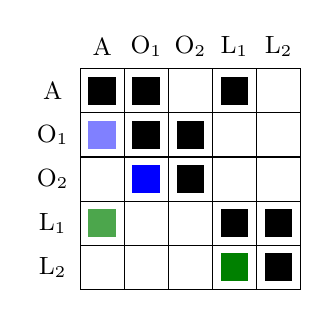
\begin{tikzpicture}
	\begin{scope}[shift={(0,0)},scale=.7]
        %\node  at (2.0,5.1) {$\textit{From}$}; 	
		\node  at (0.4,4.4) {\small$\text{A}$};
		\node  at (1.2,4.4) {\small$\text{O}_1$}; 
		\node  at (2.0,4.4) {\small$\text{O}_2$};
		 
		\node  at (2.8,4.4) {\small$\text{L}_1$}; 	
		\node  at (3.6,4.4) {\small$\text{L}_2$}; 

        %\node[rotate=90]  at (-1.3,2.0) {$\textit{To}$}; 
		\node  at (-0.5,3.6) {\small$\text{A}$}; 
		\node  at (-0.5,2.8) {\small$\text{O}_1$}; 
  	    \node  at (-0.5,2.0) {\small$\text{O}_2$};
  	     	
		\node  at (-0.5,1.2) {\small$\text{L}_1$};
		\node  at (-0.5,0.4) {\small$\text{L}_2$}; 


		\node[fill=black,scale=1.5] at (0.4,3.6) (description) {};
		\node[fill=black,scale=1.5] at (1.2,3.6) (description) {};
		\node[fill=black,scale=1.5] at (2.8,3.6) (description) {};
  
		\node[fill=blue!50 ,scale=1.5] at (0.4,2.8) (description) {};
		\node[fill=black   ,scale=1.5] at (1.2,2.8) (description) {};
		\node[fill=black   ,scale=1.5] at (2.0,2.8) (description) {};
  
		\node[fill=blue!100 ,scale=1.5] at (1.2,2.0) (description) {};
		\node[fill=black   ,scale=1.5] at (2.0,2.0) (description) {};
		%\node[fill=black   ,scale=1.5] at (2.8,2.0) (description) {};
  
		\node[fill=black     ,scale=1.5] at (2.0,2.0) (description) {};
		%\node[fill=black    ,scale=1.5] at (2.8,2.0) (description) {};

		\node[fill=Green!70 ,scale=1.5] at (0.4,1.2) (description) {};
		\node[fill=black    ,scale=1.5] at (2.8,1.2) (description) {};
		\node[fill=black    ,scale=1.5] at (3.6,1.2) (description) {};
  
  		\node[fill=Green!100 ,scale=1.5] at (2.8,0.4) (description) {};
  		\node[fill=black     ,scale=1.5] at (3.6,0.4) (description) {};
    	%\node[fill=black     ,scale=1.5] at (4.4,1.2) (description) {};


        \draw[step=.8, black] (0,0) grid (4,4);  
        %\draw[black,very thick] (0,0) rectangle (3,3); 
	\end{scope}
\end{tikzpicture}
\end{minipage}
\noindent\begin{minipage}[t]{0.4\linewidth}%
\centering
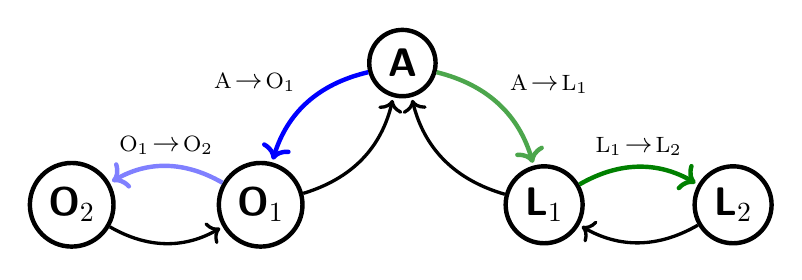
\begin{tikzpicture}[scale=0.6,->,shorten >=1pt,auto,
                        ultra thick,main node/.style={circle,draw,font=\sffamily\Large\bfseries}]
      \node[main node] (A) at (0,0) {A};
      \node[main node] (O1) at (-3,-3) {$\text{O}_1$};
      \node[main node] (O2) at (-7,-3) {$\text{O}_2$};
      \node[main node] (L1) at (3,-3) {$\text{L}_1$ };
      \node[main node] (L2) at (7,-3) {$\text{L}_2$ };

\begin{scope}[ 
    shorten > = 1pt,
node distance = 3cm and 4cm,
    el/.style = {inner sep=2pt, align=left, sloped},
every label/.append style = {font=\tiny}      ]
      \path[->,ultra thick,blue!100] (A) edge [bend right] node [above left] {$\color{black}{\footnotesize{\too{A}{$\text{O}_1$}}}$} (O1);
      \path[->,very thick] (O1) edge [bend right] node [left] {} (A);      
    %
    \path[->,ultra thick,Green!70] (A) edge [bend left] node [above right]  {$\color{black}{\footnotesize{\too{A}{$\text{L}_1$}}}$} (L1);
    \path[->,very thick] (L1) edge [bend left] node [right] {} (A);
    %
    \path[->,ultra thick,Green!100] (L1) edge [bend left] node [above]  {$\color{black}{\footnotesize{\too{$\text{L}_1$}{$\text{L}_2$}}}$} (L2);
      \path[->,very thick] (L2) edge [bend left] node [right] {} (L1);

      \path[->,ultra thick,blue!50] (O1) edge [bend right] node [above]  {$\color{black}{\footnotesize{\too{$\text{O}_1$}{$\text{O}_2$}}}$} (O2);
      \path[->,very thick] (O2) edge [bend right] node [above] {} (O1);

    \end{scope}
    \end{tikzpicture}
\end{minipage}
\caption{
The operator $\bb{A}$ is visualized (left) for the $5$PR model, which includes atmosphere ($\text{A}$), two ocean  reservoirs($\text{O}_1$ and $\text{O}_2$), and two land  reservoirs ($\text{L}_1$ and $\text{L}_2$). A graphically representation of the connectivity of the reservoirs (right) is shown with the unknown carbon mass transfer rates denoted, for example, $\text{O}_1 \! \to  \! \text{O}_2$ corresponds to the entry $\bb{A}_{3,2}$. The other model configuration $3$SR and $4$PR can all be considered as subsets of the more complex $5$PR model configuration. $\bb{A}$ is symmetric in its non-zero pattern, but not in its values.
}
\label{fig:1}
\end{figure}


Denote the nonzero strictly lower-triangular indices of $\bb{A}$ as $\mathcal{I}=\{(i,j):\bb{A}_{ij}\neq 0,i>j\}$.
For all model configurations outlined, applying conditions in~\eqref{eq:clim_model.2} and~\eqref{eq:clim_model.3}, the closed-form solutions for the upper triangular values of the restricted operator are
%
\begin{align} \label{eq:clim_model.4}
	\bb{A}_{ji} = \bb{A}_{ij}  \frac{\bb{m}^{\text{eq}}_j}{\bb{m}^{\text{eq}}_i} \; \forall \; (i,j) \in \mathcal{I}, \; \text{and} \;  \bb{A}_{ii}= -\sum_{j=1,j\neq i}^p \bb{A}_{ij}.
\end{align}
%
The unknown parameters necessary for defining the restricted operator include the strictly lower triangular nonzero values $\bb{A}_{ij}$ for all $(i,j) \in \mathcal{I}$ and the ratios of the equilibrium masses $\bb{m}^{\text{eq}}$. 
For a predefined sequence of emissions we denote the carbon-cycle simulation of length $T$ as   
%
\begin{align} \label{eq:clim_model.5}
	\bb{M}[\bb{A}] := [ \bb{m}^{1},\bb{m}^{2},\ldots,\bb{m}^{T} ], 
\end{align}
%
where $\bb{m}^{t}$ is defined as per \eqref{eq:clim_model.1}. 
We utilize acronyms depicted in Figure~\ref{fig:1} to refer to specific reservoirs; for instance, $\bb{M}[\bb{A}]^{t}_{\text{O}_2}$ represents the content of the $\text{O}_2$ reservoir at time $t$.
Throughout this work, our simulations are exclusively use atmospheric emissions, meaning $e_{\text{A}}^t$ is non-zero only when emissions are present at time $t$, while all other entries are zero.
Notice that only the ratios of $\bb{m}^{\text{eq}}$ are relevant in the definition of $\bb{A}$.
It is important to note that in defining $\bb{A}$, only the ratios of $\bb{m}^{\text{eq}}$ are relevant. 
By simplifying the problem and setting $\bb{m}^{\text{eq}}$ to the preindustrial values found in Table~\ref{tab:1} (see, e.g.,~\cite{2431585063dd4b78b890f885bb19642e} and reference therein for further details), we reduce the unknown parameters to the non-zero values in the strictly lower-triangular matrix $\bb{A}$ (as seen in Figure~\ref{eq:clim_model.1}). 
For the given model configurations, this corresponds to $n-1$ parameters.
The time-stepping scheme using for the simulation is explicit Euler. [say more about stablity] 
%
\begin{table}[t]
\centering
\small
\begin{tabular}{ccccccc}
\multirow{2}{*}{Configuration} & 
\multicolumn{5}{c}{Equilibrium Masses (GtC) \vspace{0.2em}}\\   &
$\bb{m}_{\text{A}}^{{\text{eq}}} $&
$\bb{m}_{\text{O}_1}^{{\text{eq}}}$&
$\bb{m}_{\text{O}_2}^{{\text{eq}}}$&
$\bb{m}_{\text{L}_1}^{{\text{eq}}}$&
$\bb{m}_{\text{L}_2}^{{\text{eq}}}$& \vspace{0.5em}\\
%
\toprule
\toprule
\textbf{3SR} & 
    589 & 900 & 37,100 & - & - \\
    \textbf{4PR} & 
    589 & 900 & 37,100 & 2,500 & - \\
    \textbf{5PR} & 
    589 & 900 & 37,100 & 550 & 1,950 \\
\end{tabular}
\label{tab:1}
\caption{Equilibrium masses in the different carbon reservoirs are shown for each configuration. For all configurations, $\text{O}_1$ and $\text{O}_2$ represent the upper and lower-ocean, respectively. In the $4$PR model, $\text{L}_1$ denotes the total land-biosphere equilibrium mass, while the $5$PR configuration subdivides the land-biosphere into vegetation $\text{L}_1$ and soils $\text{L}_2$. These masses correspond to the 1765 conditions, when the Earth's carbon cycle is assumed to be at equilibrium (for details, refer to \cite{2431585063dd4b78b890f885bb19642e} and the references therein).
    }
\label{tab:1}
\end{table}



%%%%%%%%%%%%%%%%%%%%%%%%%%%%%%%%%%%%%%%%%%%%%%%
\subsection{Estimation Procedure} 
%%%%%%%%%%%%%%%%%%%%%%%%%%%%%%%%%%%%%%%%%%%%%%%
Our proposed estimation procedure optimizes the $n-1$ parameters of $\bb{A}$ by (1) minimizing the discrepancy between the our simulations and publicly available benchmarks,\footnote{see,~\url{https://climatehomes.unibe.ch/~joos/IRF_Intercomparison/results.html} for details} while (2) penalizing solutions that do not conform to observed physical principles.
The adopted simulation benchmarks are based on the work of~\cite{joos2013carbon}, in which various Earth System Models were used to simulate the decay of a $100$ GtC pulse introduced into the atmosphere during preindustrial times when the Earth's carbon-cycle is assumed to be at equilibrium.
Figure~\ref{fig:2} showcases the benchmark dataset for the various models.
We enforce three physical principles: (i) reducing variability in parameter estimates, (ii) minimizing dynamic timescales, and (iii) ensuring an approximately equal cumulative pulse emission flux from the atmosphere to both ocean and land biosphere reservoirs shortly after the pulse.
We first begin with formalizing these physical principals, encoding them in in three district penalty functions $q_1,q_2$ and $q_3$. 
Subsequently, we outline the comprehensive optimization process for the estimation procedure.

[more text here]
\newpage

We employ three scenarios to estimate the operator parameters: the multi-modal mean and two standard deviation extrema, denoted as $\mathcal{B}:=\{\mu,\mu^+,\mu^-\}$, respectively (see Figure~\ref{fig:2} for details). 
Given a benchmark $b \in \mathcal{B}$, we obtain varying estimates of $\bb{A}^{b}$ for each $b$. 
The operator estimate $\bb{A}^{b}$ should be stable in the sense that the estimated parameters across the benchmarks should have similar values.
To reduce the variability amongst the estimates $\bb{A}^{b}$, we penalize the difference between the parameter estimates with respect to $b=\mu$.
We encode this attribute in the penalty function 
%
\begin{align}\label{eq:clim_model.6}
	q_1(\bb{A}^b) := \left \| \bb{a}^\mu - \bb{a}^b \right \|_2 ,\; \text{where} \; \bb{a}^b:= \{\bb{A}^b_{ij}: \forall (i,j) \in \mathcal{I}      \},
\end{align}
%
This penalty function results in a non-separable dependency between the parameter estimates. 
This dependency plays a critical role in constraining the range of potential operators that best fit the decay of atmospheric pulse emissions (see, e.g., Section X for further details.)
 %
\begin{figure}[t]
    \centering
    \includegraphics[width=\textwidth]{fig/pulse.png}
    \caption{
    The decay of a 100 GtC pulse of emissions in the pre-industrial atmosphere (1765) was analyzed using various Earth System Models of differing complexities.
    This data is based on a series of controlled simulations conducted by~\cite{joos2013carbon}.
    For further details on the simulations and model descriptions, we refer the reader to the cited reference. The multi-modal mean of the simulations, denoted by $\mu$, along with the two standard deviations above and below the mean, are represented by $\mu^+$ and $\mu^-$, respectively.
     }
    \label{fig:2}
\end{figure}

 
The proposed carbon-cycle model, along with various configurations, is a simplified approximation of a considerably more complex system. 
Rather than attempting to model processes across the spectrum of timescales, our goal here is to model the salient responses that play a significant role in the shortest timescales. 
To penalize large dynamic timescales we encourage increasing eigenvalues magnitudes of $\bb{A}^b$, which corresponds to the penalty function
%
\begin{align}\label{eq:clim_model.7}
	q_1(\bb{A}^b) := \frac{1}{n} \tr{\bb{A}^b} = \frac{1}{n}\sum_{i=1}^n \bb{\lambda}_i(\bb{A}^b).
\end{align}
%
Since the eigenvalues of the operator are strictly real and non-positive, the corresponding penalty function is strictly non-positive. 
This approach is further motivated by the economic model (see Section X), in which long-term damages hold little significance due to the discounting factor.

Following the pulse event, it is expected that the total pulse flux will be equally distributed between the ocean and land reservoirs in the short term. 
This assumption is corroborated by~\cite{joos2013carbon}, where the simulation of a $100$ GtC atmospheric emission (during preindustrial times) leads to an approximately equal partition of $60$ GtC of cumulative emissions in the ocean and land carbon reservoirs within $40$ to $60$ years after the pulse. 
We incorporate this observation by limiting the cumulative flux discrepancy between the ocean and land reservoirs using the penalty function
\begin{align}\label{eq:clim_model.8}
	q_3(\bb{A}^b) := \left \| \frac{\bb{M}_{\text{O}}^{t_e}[\bb{A}^b] - \bb{M}_{\text{L}}^{t_e}[\bb{A}^b] }{\bb{M}_{\text{O}}^{t_e}[\bb{A}^b] + \bb{M}_{\text{L}}^{t_e}[\bb{A}^b] }\right \|_2,
\end{align}
%
where $\bb{M}^{t_e}_{\text{O}}[\bb{A}^b]$ is the total mass of all ocean reservoirs (and similarly, the superscript $\text{L}$ denotes all land biosphere reservoirs) at time $t_e$. 
In our experiments, we set $t_e=50$.

 
Let $\bb{y}^b$ represent the benchmark dataset of atmospheric carbon mass for the decaying $100$ GtC pulse, spanning a total of $T$ years after the pulse. 
In this pulse scenario, the emissions are defined as $\bb{e}^1_\text{A}=100$ and zero for all other cases. 
Moreover, since we begin with preindustrial conditions, it follows that $\bb{m}^{0}=\bb{m}^{\text{eq}}$.
Given the non-negative tuning coefficients $\rho_1$, $\rho_2$, and $\rho_3$, which correspond to each penalty function, the proposed estimation procedure seeks optimize
 %
 \begin{align}\label{eq:clim_model.9}
 	\minimize{ \substack{\{ \bb{A}^{b} \\ b  } \}   \; \forall\; b \in \mathcal{B} }  \left\{ \; \sum_{v \in \mathcal{B}} 
 		 \frac{1}{T} \left \| \bb{M}_{\text{A}}[\bb{A}^b] - \bb{y}^b  \right\|_2  + 
 		 \rho_1 q_1(\bb{A}^b,\bb{A}^\mu) +  
 		 \rho_1 q_2(\bb{A}^b) +   
 		 \rho_3 q_3(\bb{A}^b)  
 		 \right\},
 \end{align}
 %
where $\bb{M}_{\text{A}}[\bb{A}^b]$ represents the simulated values of atmospheric carbon content for the time period ranging from $t=1$ to $T$.


[Say more about optimization method used ... and bounds of optimizer. The max percentage transfer of mass form one reservoir to the next is 15\%]

 


\subsection{Calibration}



\begin{table}[ht]
\centering
\small
\begin{tabular}{cccccc}
\multirow{2}{*}{Configuration} & 
\multicolumn{5}{c}{Mass Flow Coefficients (Expressed as \%)  \vspace{0.2em}}\\   &
$\bb{A}_{21} / \footnotesize{\too{$\text{A}$}{$\text{O}_1$}}$&
$\bb{A}_{32} / \footnotesize{\too{$\text{O}_1$}{$\text{O}_2$}}$&
$\bb{A}_{41} / \footnotesize{\too{$\text{A}$}{$\text{L}_1$}}$& 
$\bb{A}_{54} / \footnotesize{\too{$\text{L}_1$}{$\text{L}_2$}}$\\ 
%
\toprule
\toprule
    \textbf{3SR}& 15.00|14.98|14.99 &  0.14|0.22|0.37 & &\\
    \textbf{4PR}& 2.17|0.81|2.57 & 0.05|0.04|0.11 & 0.15|0.74|1.81 & & \\
    \textbf{5PR}& 0.4|0.85|2.41 & 0.05|0.04|0.11 & 0.41|0.91|2.52 & 12.96|13.21|12.98 & \\
    \end{tabular}
    \caption{The umbers here are presented as \% (ie, they should be divided by 100). The number follow the format ($\mu^+,\mu,\mu^-$)}
\end{table}



\begin{figure}[b]
    \centering
    \includegraphics[width=\textwidth]{fig/analyse_pen.png}
    \caption{Objective Value Components (penalties) }
    %\label{fig:my_label}
\end{figure}


\begin{figure}
    \centering
    \includegraphics[width=\textwidth]{fig/analyse_cum_flux_flux.png}
    \caption{Pulse Cumulative FLux per model}
    \label{fig:selection_best}
\end{figure}


\begin{figure}
    \centering
    \includegraphics[width=\textwidth]{fig/analyse_err.png}
    \caption{Pulse Fit Error}
    \label{fig:selection_best}
\end{figure}




\section{Simulation}


\subsection{Synthetic Scenarios}

\begin{figure}
    \centering
    \includegraphics[width=\textwidth]{fig/sim_pulse.png}
    \caption{Joos 100 GtC Pulse (symmetry of the response to a negative pulse given due to linearity of the model )}
    %\label{fig:selection_best}
\end{figure}




\subsection{CMIP}

\begin{figure}
    \centering
    \includegraphics[width=\textwidth]{fig/simulate_cmip_conc.png}
    \caption{CMIP Concentrations}
    %\label{fig:selection_best}
\end{figure}



\begin{figure}
    \centering
    \includegraphics[width=\textwidth]{fig/simulate_cmip_temp.png}
    \caption{CMIP Temprature}
    %\label{fig:selection_best}
\end{figure}


\subsection{MacDougall}



\begin{figure}
    \centering
    \includegraphics[width=\textwidth]{fig/simulate_macdougall_1.png}
    \caption{MacDougall 1, Note $t_c$ is the time at which the emission of MacDougall end and the system is left to "coast". }
    %\label{fig:selection_best}
\end{figure}


\begin{figure}
    \centering
    \includegraphics[width=\textwidth]{fig/simulate_macdougall_2.png}
    \caption{MacDougall 2: System response after emission have stopped.}
    %\label{fig:selection_best}
\end{figure}



\appendix


\clearpage
% with BibTeX
\bibliography{references.bib}

\end{document}

%%% Local Variables:
%%% mode: latex
%%% TeX-master: t
%%% End: